\chapter[Software]{Software}

\section[WebService]{WebService}

\subsection{Requisitos do Projeto}

\subsubsection{Cadastrar usuário}

\textbf{Dado} que a API receba uma requisição para cadastrar um novo usuário

\textbf{E} todos os campos do usuário sejam válidos

\textbf{Então} o usuário deve ser cadastrado.

\subsubsection{Autenticar usuário}

\textbf{Dado} que a API receba uma requisição para autenticar um usuário

\textbf{E} todos os campos do usuário sejam válidos

\textbf{Então} o token correspondente ao usuário deve ser gerado.

\subsubsection{Realizar Pagamento}

\textbf{Dado} que a API receba uma requisição para registrar um pagamento

\textbf{E} os dados de pagamento sejam validados junto a API do PagSeguro

\textbf{Então} a transação deve ser efetivada.

\subsubsection{Gerar Qrcode}

\textbf{Dado} que a API receba uma notificação da API do PagSeguro

\textbf{E} o status da transação seja alterado para \textit{paga}

\textbf{Então} deve ser gerado um QrCode.

\subsubsection{Validar qrcode}

\textbf{Dado} que a API receba uma requisição com um QrCode

\textbf{E} o QrCode seja válido

\textbf{Então} deve ser retornado as informações referente ao QrCode.

\subsubsection{Mostrar chopps}

\textbf{Dado} que a API receba uma requisição para mostrar os chopps de um usuário

\textbf{E} o usuário esteja logado

\textbf{Então} deve ser retornado os chopps referentes a esse usuário.

\subsubsection{Salvar dados dos sensores}

\textbf{Dado} que a API receba uma requisição para salvar os dados dos sensores

\textbf{E} os dados sejam válidos

\textbf{Então} os dados devem ser salvos.

\subsubsection{Mostrar dados dos sensores}

\textbf{Dado} que a API receba uma requisição para mostrar os dados dos sensores

\textbf{E} o usuário seja um administrador

\textbf{Então} os dados devem ser mostrados.

\subsection{Projeto}

A demanda do problema exige que diferentes hardwares se integrem com uma
mesma base de dados. Fundamentalmente, o Smartphone do usuário realiza a compra, e
a máquina deve validar o QrCode para que o usuário consuma o chopp.

Para solucionar essa demanda foi proposto uma arquitetura orientada a serviços
(SOA), tal que uma webservice REST seja responsável pela persistência e autenticação de todos os
dados relevantes do sistema. Sendo assim esse WebService será responsável por se comunicar com
todos os outros subsistemas.

O modelo de domínio abaixo traz uma visão inicial das entidades presentes no sistema.

\begin{figure}[H]
    \centering
    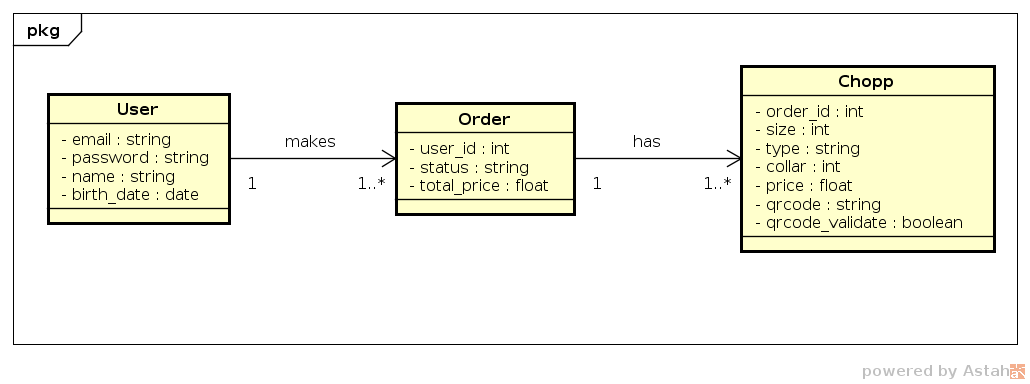
\includegraphics[scale= 0.5]{figuras/modelo-dominio.png}
    \caption{Modelo de Domínio. Fonte: Própria.}
    \label{modelagem}
\end{figure}

\subsection{Solução Adotada}

Visto que é requisito primordial do sistema o checkout de pagamentos via cartão de cŕedito, a
tecnologia escolhida para implementação desse WebService foi o framework 
Ruby On Rails\footnote{\url{http://rubyonrails.org/}}, pois a API de pagamentos do PagSeguro
fornece suporte a essa tecnologia. A versão utilizada do Ruby foi a versão 2.3.0 e o Rails a versão 5.0.5.

\subsubsection[Arquitetura]{Arquitetura}

\subsubsubsection{Models}

As classes modelos no Rails representam as entidades e seus relacionamentos, e são responsáveis pelo gerenciamento dos dados
no banco. O diagrama de classes abaixo representa as classes modelos do sistema:

\begin{figure}[H]
    \centering
    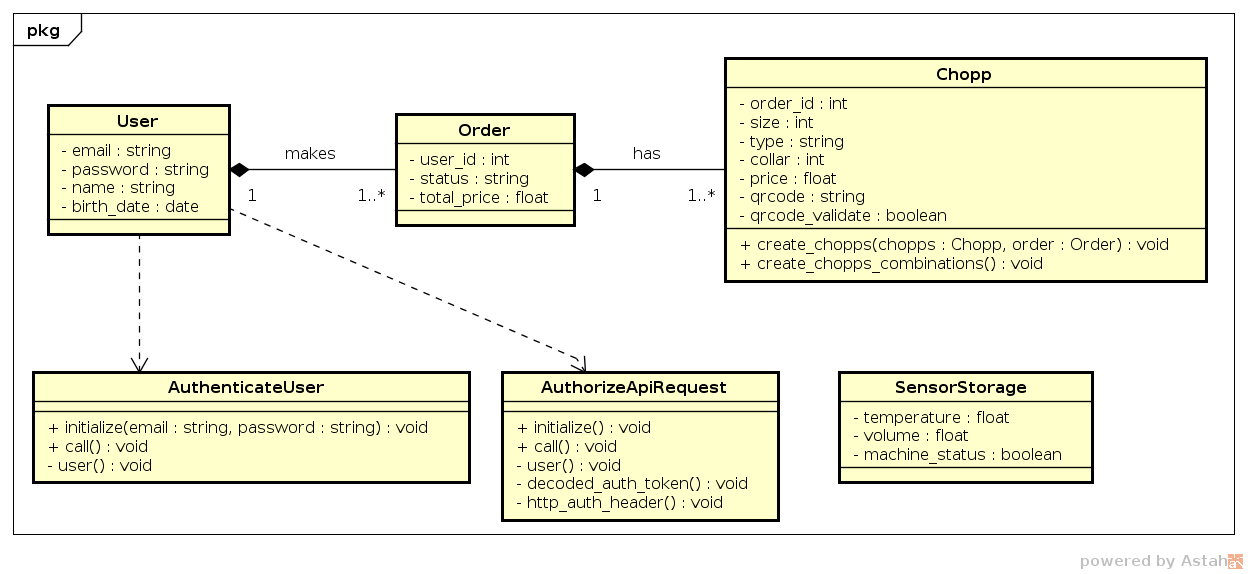
\includegraphics[scale= 0.5]{figuras/diagrama-models.png}
    \caption{Diagrama de Classes - Models. Fonte: Própria.}
    \label{modelagem}
\end{figure}

\begin{itemize}
    \item \textbf{User:} A classe \textit{User} guarda as informações referentes a um usuário.
    \item \textbf{Order:} A classe \textit{Order} guarda as informações referentes a um pedido
    de um usuário específico. 
    \item \textbf{Chopp:} A classe \textit{Chopp} guarda as informações referentes a um chopp
    de um pedido específico.
    \item \textbf{SensorStorage:} A classe \textit{SensorStorage} guarda as informações referentes
    aos valores lidos dos sensores do módulo embarcado.
    \item \textbf{AuthenticateUser:} A classe \textit{AuthenticateUser} é responsável por autenticar um usuário
    na base de dados.
    \item \textbf{AuthorizeApiRequest:} A classe \textit{AuthorizeApiRequest} é reponsável por 
    decodificar determinado token de autenticação.
\end{itemize}

\subsubsubsection{Controllers}

As classes controladoras no Rails são responsáveis por se comunicar com as classes modelos, e são elas que lidam com
requisições web do usuário. O diagrama de classes abaixo representa as classes controladoras do sistema:

\begin{figure}[H]
    \centering
    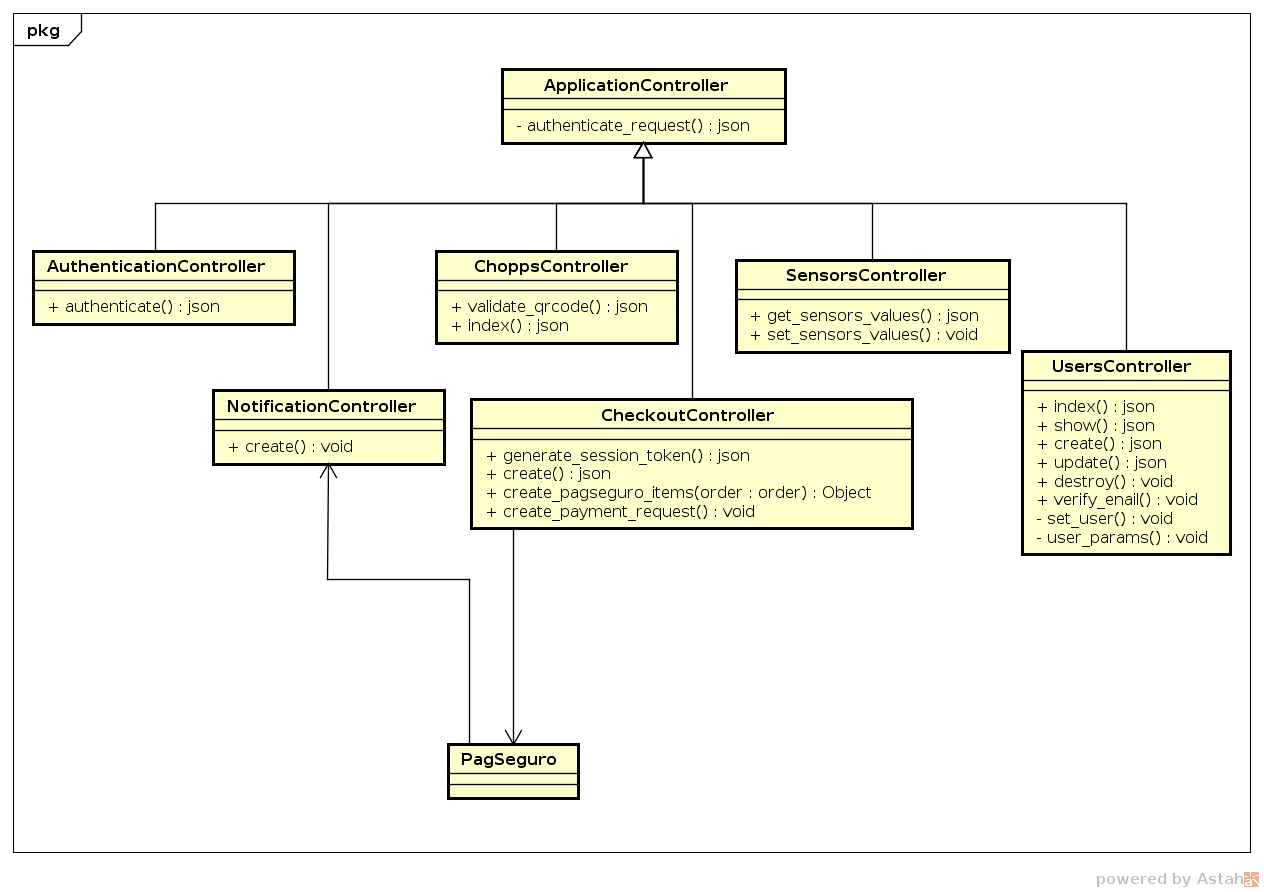
\includegraphics[scale= 0.5]{figuras/diagrama-controllers.png}
    \caption{Diagrama de Classes - Controllers. Fonte: Própria.}
    \label{modelagem}
\end{figure}

\begin{itemize}
    \item \textbf{ApplicationController:} A classe \textit{ApplicationController} é a controladora padrão do Rails
    e todas as outras controladoras são herdadas a partir desta.
    \item \textbf{UsersController:} A classe \textit{UsersController} é responsável por enviar e receber os dados dos usuários.
    \item \textbf{AuthenticationController:} A classe \textit{AuthenticationController} é reponsável por receber os dados do usuário
    e realizar a autenticação.
    \item \textbf{ChoppsController:} A classe \textit{ChoppsController} é responsável por enviar e receber os dados dos chopps.
    \item \textbf{SensorsController:} A classe \textit{SensorsController} é responsável por enviar e receber os dados dos sensores.
    \item \textbf{CheckoutController:} A classe \textit{CheckoutController} é responsável por receber os dados de pagamento e enviar
    a API do PagSeguro.
    \item \textbf{NotificationController:} A classe \textit{NotificationController} é reponsável por receber notificações da API
    do PagSeguro quando uma transação muda de status.
    \item \textbf{PagSeguro:} Entidade que representa a API do PagSeguro.
\end{itemize}

\subsection{Casos de Teste}

Para testar o funcionamento correto da API foi utilizada a ferramenta \textit{Rspec}, que nos permite
testar a aplicação unitariamente, através de testes unitários. Com este tipo de teste é possível testar
o comportamento de cada método. A imagem abaixo mostra a cobertura de testes: 

\begin{figure}[H]
    \centering
    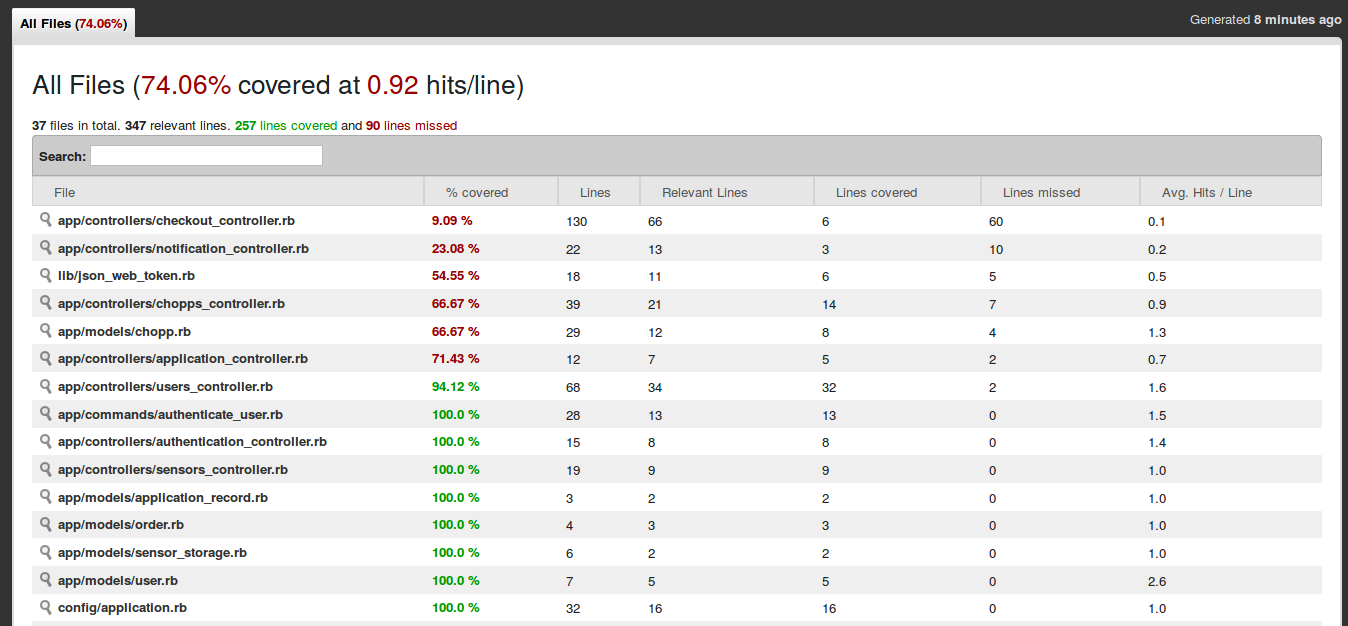
\includegraphics[scale= 0.3]{figuras/Cobertura.png}
    \caption{Cobertura de Testes. Fonte: Própria.}
    \label{modelagem}
\end{figure}

Como a demanda do projeto é muito grande, não foi possível testar todos os métodos unitariamente, logo,
também foi utilizada a ferramenta \textit{Postman}. Essa ferramenta nos permite testar se a API está respondendo
corretamente as requisições.

\subsection{Gerência e Configuração}

\begin{itemize}
    \item \textbf{Deploy:} Para hospedagem do WebService foi usado o \textit{Heroku}\footnote{\url{https://www.heroku.com/}}.
    As vantagens em utilizar essa plataforma estão no custo, por ser uma ferramenta grátis e na facilidade em realizar o deploy.
    \item \textbf{Integração Contínua:} Para a integração contínua foi utilizada a ferramenta 
    \textit{TravisCI}. Com esta ferramenta, a cada commit no repositório todos os testes são executados
    automatizadamente, e assim é possivel verificar se aquele commit quebrou a build.
\end{itemize}

\section[Aplicativo Mobile]{Aplicativo Mobile}

Para compra e gerenciamento dos cupons de \textit{chopp}, torna-se necessário um aplicativo \textit{mobile} de forma que seja facilitado a acessibilidade para os usuários.

\subsection{Requisitos do Projeto}

\subsubsection{Comprar Chopp}

\textbf{Dado} que o usuário esteja logado

\textbf{Quando} tenha iniciado a compra de um chopp

\textbf{Então} deve ser possível ver as preferências de chope(colarinho, quantidades discretas e pré-definidas)

\subsubsection{Cadastrar Usuário}

\textbf{Dado} que o usuário tente entrar no sistema 

\textbf{E} ainda não tenha se cadastrado

\textbf{Quando} tenha iniciado o aplicativo

\textbf{Então} terá disponível um formulário com email e senha para cadastro

\subsubsection{Confirmar Cadastro}

\textbf{Dada} que o usuário já tenha se cadastrado

\textbf{E} recebido um email com link de confirmação

\textbf{Quando} clicar no link

\textbf{Então} deverá ser levado a uma mensagem de confirmação

\textbf{E} deve ser possível se autenticar no sistema.

\subsubsection{Finalizar Compra}

\textbf{Dado} que o usuário já esteja cadastrado no sistema

\textbf{E} tenha clicado para comprar um chopp

\textbf{E} tenha acesso a internet

\textbf{Quando} finalizado a compra

\textbf{Então} deve ser possível inserir os dados do cartão de crédito

\textbf{E} ser notificado se a compra foi bem sucedida ou não

\textbf{E} em seus tickets devem estar disponíveis para uso na máquina

\subsubsection{Listar Cupons(QRCode)}

\textbf{Dado} que o usuário já tenha comprado tickets

\textbf{E} esteja autenticado no sistema

\textbf{Quando} clicar em uma opção meus tickets

\textbf{Então} deve ser possível  visualizar o QRCode que representa a unidade de chopp

\textbf{E} deverá ter disponível uma opção para usar o ticket

\textbf{E} caso já tenha sido usado o ticket, deverá sumir da lista de tickets do usuário

\subsubsection{Efetuar Compra Offline}

\textbf{Dada} a compra efetuada de um chopp

\textbf{E} um usuário offline

\textbf{Quando} o usuário clicar para usar o ticket

\textbf{Então} a máquina de chopp deve responder no sistema de interação com mensagem sucesso.

\subsubsection{Visualizar Cupons(QRCode)}

\textbf{Dado} que o usuário tenha comprado tickets

\textbf{Quando} entrar na tela de visualização de tickets

\textbf{Então} deve ser possível ver os tickets comprados segundo as preferências

\textbf{E} poder escolher qual queira consumir

\subsection{Projeto}

De acordo com os critérios observados do público alvo e do contexto considerado, pensou-se em um aplicativo mobile que se comunica com um Web Service para realizar as operações descritas na especificação acima.

\subsection{Solução Adotada}

Para entendimento da solução implementada, será discutido nos tópicos seguintes sobre a arquitetura e os resultados da implementação.

\subsubsection{Arquitetura}

Por fim, decidiu-se desenvolver um aplicativo multiplataforma utilizando o \textit{framework Ionic 3}, baseado em \textit{Angular 4}, uma biblioteca Typescript que facilita a criação de aplicativos \textit{Web} e \textit{Mobile}. Conforme \cite{ionic}, Ionic é um \textit{framework open source} para desenvolvimento de aplicativos \textit{mobile} utilizando tecnologias web(HTML, CSS, JavaScript). O Ionic usa do poder do Angular para trabalhar com componentização, elevando o reaproveitamento de código.

\begin{figure}[!hb]
    \centering
    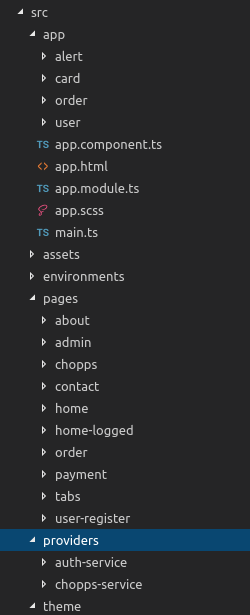
\includegraphics{figuras/ionicstructure.png}
    \caption{Estrutura de diretórios do Ionic 3.}
    \label{home-page}
\end{figure}

\subsubsection{Aplicativo}

A seguir, de acordo com os requisitos acordados, estão as imagens das principais telas do aplicativo:

\begin{figure}[!htb]
    \centering
    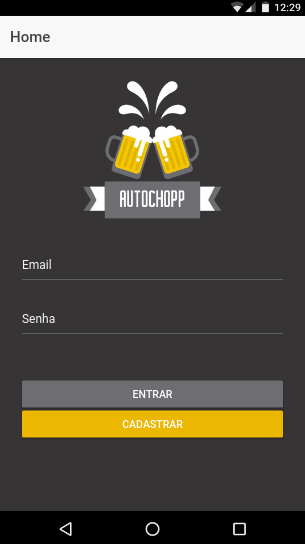
\includegraphics[scale= 0.3]{figuras/Aplicativo/home.png}
    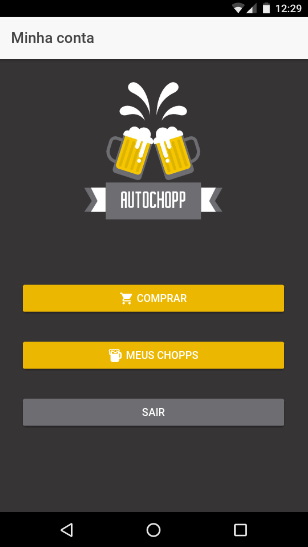
\includegraphics[scale= 0.3]{figuras/Aplicativo/home-loged.png}       
    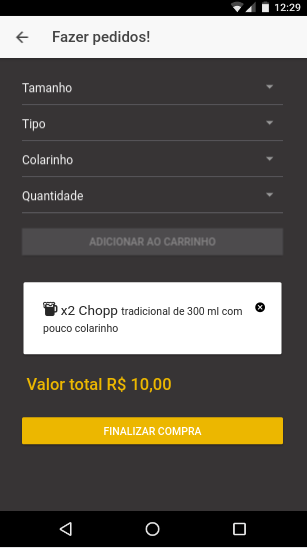
\includegraphics[scale= 0.3]{figuras/Aplicativo/compra.png}   
    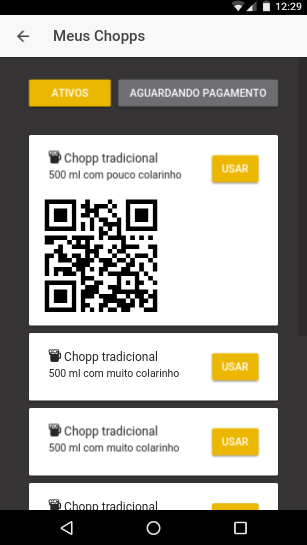
\includegraphics[scale= 0.3]{figuras/Aplicativo/chopps.png}   
    \caption{Telas do Aplicativo. Fonte: Própria.}
    \label{home-page}
\end{figure}

\subsection{Casos de Teste}

Não foram especificados casos de teste para o aplicativo \textit{mobile}, pois acredita-se que a especificação por exemplo elicitada já serve como caso de teste, uma vez que os cenários não se divergem tanto.


\section[Sistema Administrativo]{Sistema Administrativo}

O Sistema administrativo está incorporado ao aplicativo do Sistema de Compras, porém apenas usuários administradores possuem acesso. Ao utilizar o aplicativo, o usuário visualiza as seguintes informações referentes ao estado da máquina: a quantidade de chopp que a máquina possui, a temperatura de resfriamento e o status da conexão da máquina com a internet.

Esses valores são recuperados através de requisições GET ao WebService que guarda essas informações recebendo requisições POST a cada 60 seg da aplicação embarcada que lê os dados dos sensores. 

\subsection{Aplicativo}

A imagem abaixo representa a tela do usuário administrador:

\begin{figure}[!htb]
    \centering
    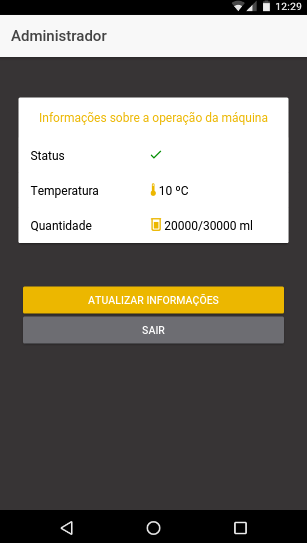
\includegraphics[scale= 0.4]{figuras/Aplicativo/admin.png}        
    \caption{Tela do Administrador. Fonte: Própria.}    
    \label{home-page}
\end{figure}


\section[Sistema de Validação de Compra]{Sistema de Validação de Compra}
\subsection[Requisitos do Projeto]{Requisitos do Projeto}
\subsubsection[Leitura de um cupom]{Leitura de um cupom}
\begin{itemize}
    \item \textbf{Dado} uma pessoa com cupons comprados
    \item \textbf{Quando} o mesmo selecionar a opção de validar um cupom da tela inicial
    \item \textbf{Então} deve ser instruído a exibir o QRCode na câmera da máquina para
    efetuar o uso do cupom
    \item \textbf{E} a máquina deve informar se a leitura ocorreu de forma correta ou não.
\end{itemize}

\subsubsection[Leitura de um cupom válido]{Leitura de um cupom válido}
\begin{itemize}
    \item \textbf{Dado} uma pessoa com um cupom válidado pelo sistema
    \item \textbf{Quando} o mesmo receber a confirmação de leitura com suceso do cupom
    \item \textbf{Então} deve ser instruído a pegar o copo na gaveta e posicionar o copo
    no suporte
    \item \textbf{E} aguardar o processo de serventia do chopp conforme as preferências.
\end{itemize}

\subsubsection[Leitura de um cupom inválido]{Leitura de um cupom inválido}
\begin{itemize}
    \item \textbf{Dado} uma pessoa com um cupom invalidado pelo sistema
    \item \textbf{Quando} o mesmo receber a confirmação de leitura sem suceso do cupom
    \item \textbf{Então} deve ser instruído a tentar novamente a leitura do cupom
    \item \textbf{E} em caso de insucesso aguardar o sistema ser recuperado, ou entrar
    em contato com o proprietário da máquina.
\end{itemize}

\subsection[Projeto]{Projeto}
O produto exige uma forma de retirada do chopp de forma autônoma, isso implicou no desenvolvimento
de uma aplicação gráfica acoplada na máquina que servisse de forma interativa com o usuário fazendo
a validação dos cupons e servindo os chopps conforme as preferências.

\subsection[Solução Adotada]{Solução Adotada}
Por ser necessária a criação de uma aplicação que não consumisse muitos recursos, optou-se pelo
uso do \textit{framework} Kivy juntamente com a linguagem de programação Python, fornecendo
um maior suporte ao foco principal da aplicação que é a leitura e reconhecimento de cupons (QrCodes)

A solução foi instalada na própria máquina, sobre o sistema operacional padrão
da plataforma Raspberry, o Raspbian, com intuito de evitar incompatibilidade com outros
sistemas operacionais e retrabalho.

\subsubsection[Arquitetura]{Arquitetura}
Por se tratar de uma aplicação com poucas funcionalidades, dados e entidades a serem trabalhadas,
não há uma distinção entre models e controllers. O diagrama de classes presente na imagem 
\ref{classes-kivy} representa a disposição das classes do sistema.

\begin{figure}[!htb]
    \centering
    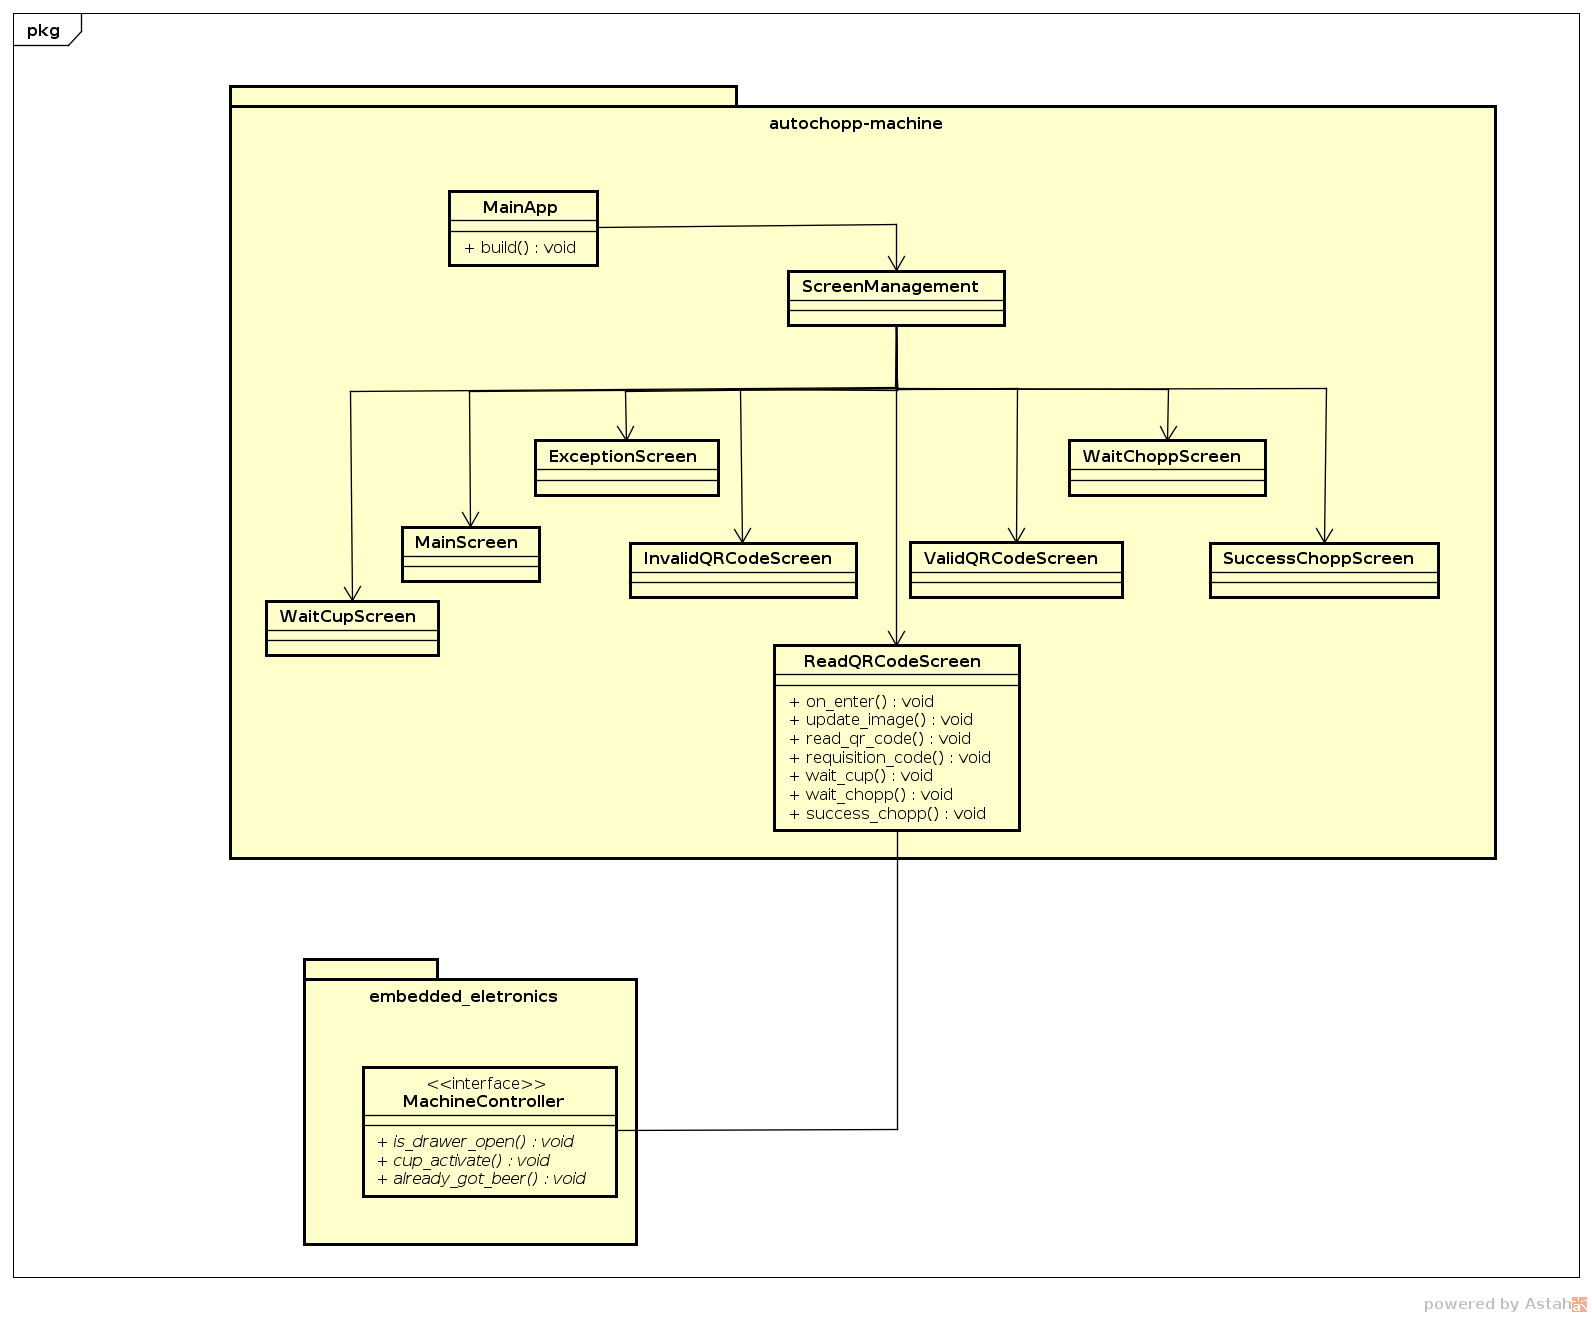
\includegraphics[scale= 0.3]{figuras/autochopp-machine-diagrama.png}        
    \caption{Diagrama de clases do sistema de validação de compras. Fonte: Própria.}
    \label{classes-kivy}
\end{figure}

Analisando o diagrama, percebe-se que a maioria das classes estão sem métodos e sem atributos,
isso acontece pelo fato de que cada tela a ser renderizada, necessita de uma classe para estar
associada. O Kivy faz uma diferenciação entre classes \textit{Screens} e classes \textit{Apps}.
A primeira se refere a classes que estão associadas a alguma tela a ser renderizada, enquanto
que as classes do segundo tipo são as responsáveis por compilar uma \textit{build} do projeto
e executar o mesmo. Nesse caso a classe do tipo \textit{App} é a classe \textit{MainApp}. Outro
ponto a ser elucidado é que a transição entre telas é gerenciado pela classe
\textit{ScreenManagement} que acopla todas as \textit{Screens} do projeto e as integra permitindo
a classe \textit{MainApp} gerar a \textit{build} das mesmas.

Além da parte gráfica e de leitura e validação de cupons, essa aplicação tem como objetivo
também a comunicação com a parte de leitura de alguns sensores para a construção do projeto.
Com isso, todos os scripts de leituras de sensores foram abrigados no pacote
\textit{embedded eletronics} criando uma interface entre as funções necessárias para o processo
de serventia de chopps e a aplicação gráfica. Tais funcionalidades são consumidas na classe
responsável pelo gerenciamento da leitura dos cupons junto a câmera.

\subsubsection{Aplicação Final}

\begin{figure}[!htb]
    \centering
    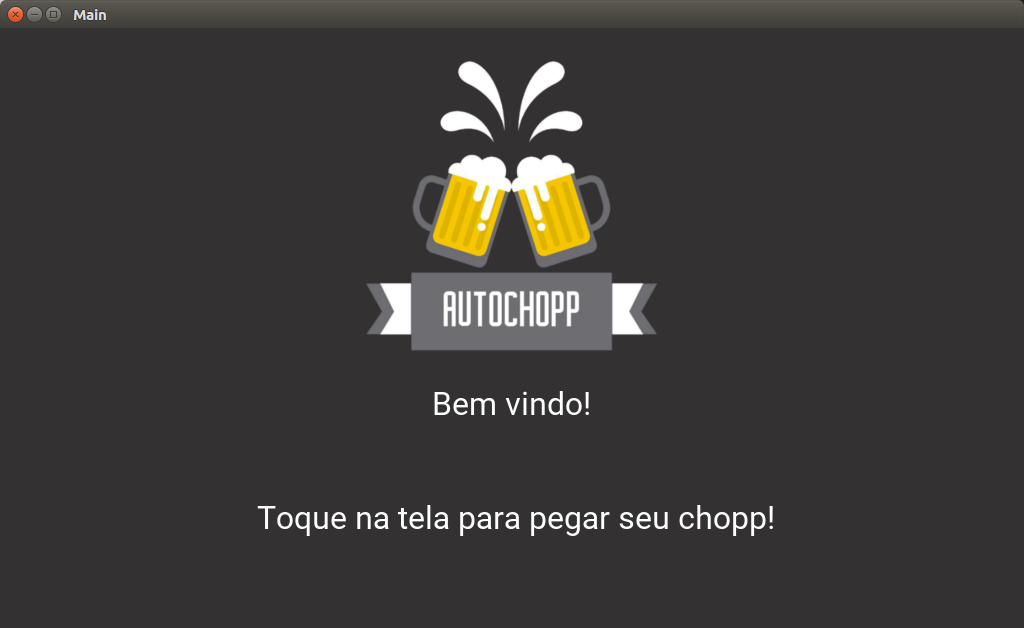
\includegraphics[scale= 0.3]{figuras/inicio.png}        
    \caption{Tela inicial. Fonte: Própria.}
    \label{classes-kivy}
\end{figure}

\begin{figure}[!htb]
    \centering
    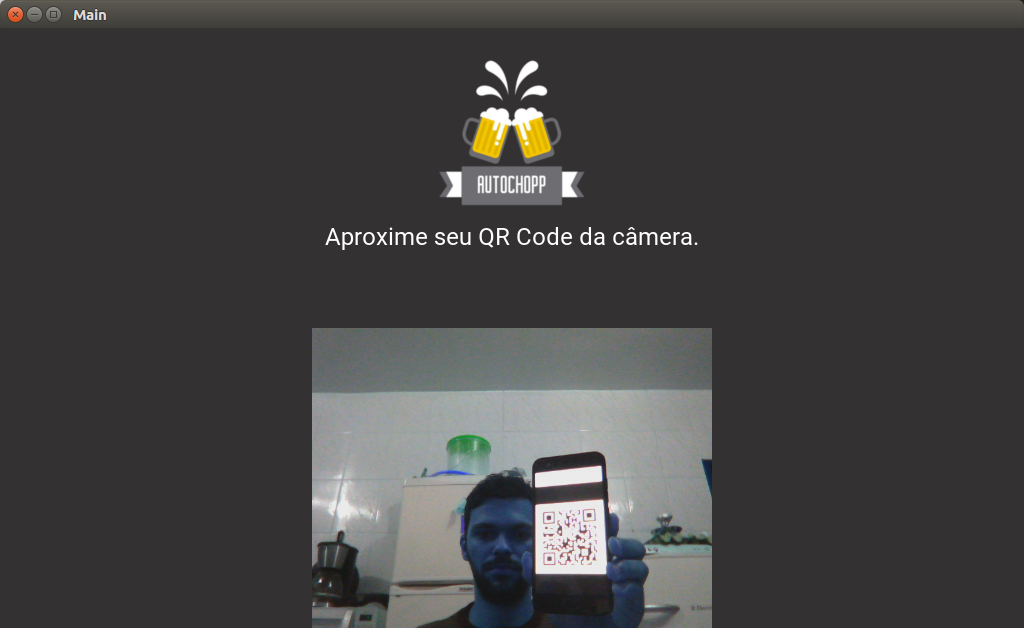
\includegraphics[scale= 0.3]{figuras/qrcode.png}        
    \caption{Tela de leitura do QR Code. Fonte: Própria.}
    \label{classes-kivy}
\end{figure}

\subsection{Casos de Teste}

\subsubsection{Leitura do Qrcode}

Para leitura do Qrcode, o usuário deve posicionar um Qrcode em frente a câmera.
Para testar esse comportamento, foi verificado se a câmera conseguia identificar a string dentro do Qrcode.

\subsubsection{Validação do Qrcode}

Para validar o Qrcode, a aplicação deve mandar uma requisição \textit{POST} ao WebService descrito anteriormente.
Para testar este comportamento, foi verificado o retorno da requisição ao WebService.

\subsubsection{Integração com o eletrônica}

Como mostra a figura \ref{classes-kivy}, a classe \textit{MachineController} é a interface que separa
a implementação dos componentes embarcados do sistema de validação de compras. Para testar o funcionamento
correto do sistema independente do módulo embarcado, foi implementado os métodos da interface com
\textit{sleeps}, que simularam o comportamento do módulo embarcado.

\section{Subsistemas integrados}

Com o objetivo de demonstrar a integração da solução, por meio da interação entre os subsistemas a partir a ação inicial 
do usuário, foram criados diagramas de sequência com duas das principais funcionalidades do sistema (Compra do chopp e 
Tiragem do chopp).


"\textit{O diagrama de sequência é um diagrama comportamental que preocupa-se com a ordem temporal em que as mensagens 
são trocadas entre os objetos envolvidos em um determinado processo.}\footnote{GUEDES, Gilleanes TA. UML 2-Uma Abordagem 
Prática-1ª Edição. Novatec Editora, 2011.}"  Partindo dessa definição, os diagramas de sequências 
foram criados, tratando os sistemas como objetos da solução de software global. Os diagramas são apresentados em seguida, 
e envolvem a interação entre WebService, Aplicativo Mobile (engloba o Sistema Administrativo), Aplicação Embarcada (Sistema de 
Validação de Compra) e API do PagSeguro, tendo como ator o usuário da solução.


\begin{figure}[!htb]
    \centering
    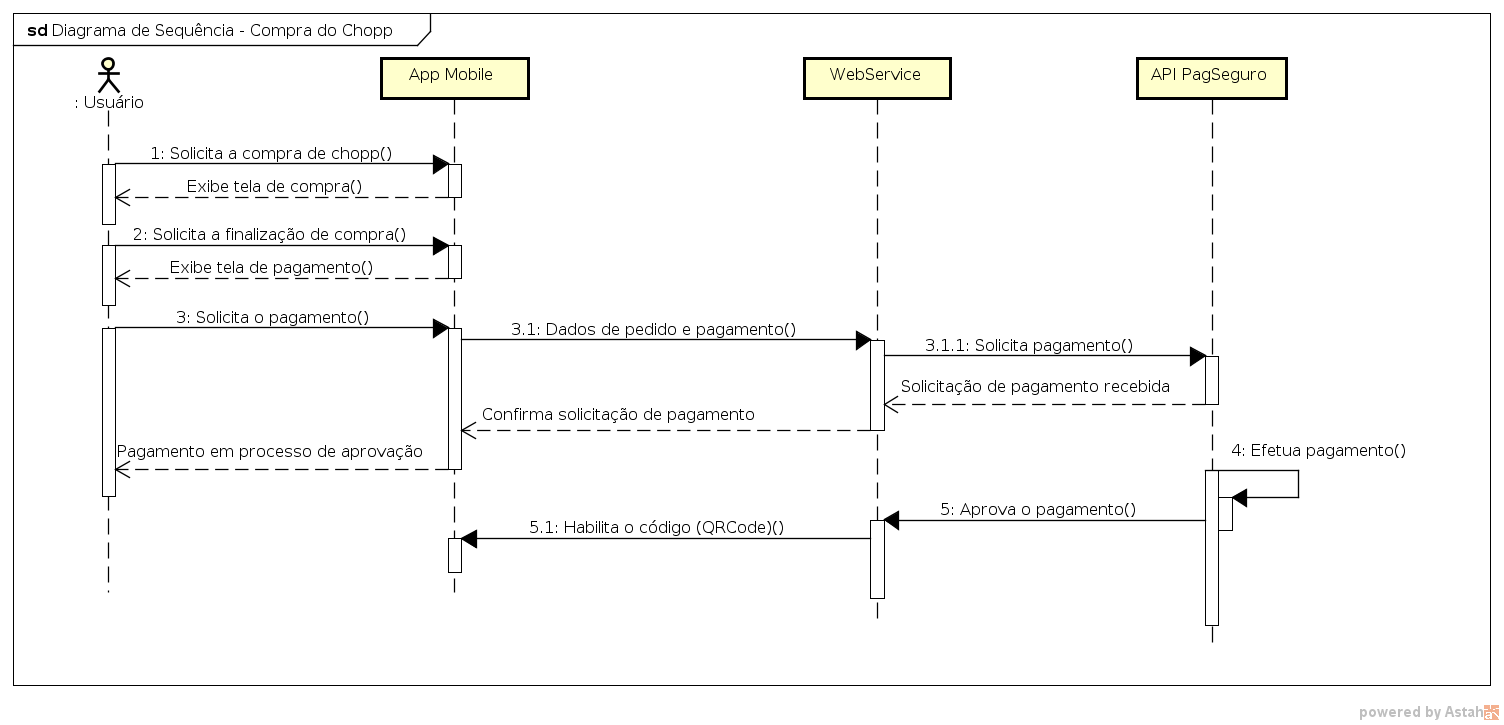
\includegraphics[scale= 0.4]{figuras/Diagrama-de-Sequencia-Compra-do-Chopp.png}        
    \caption{Diagrama de Sequência - Compra do Chopp. Fonte: Própria.}
    \label{classes-kivy}
\end{figure}

\begin{figure}[!htb]
    \centering
    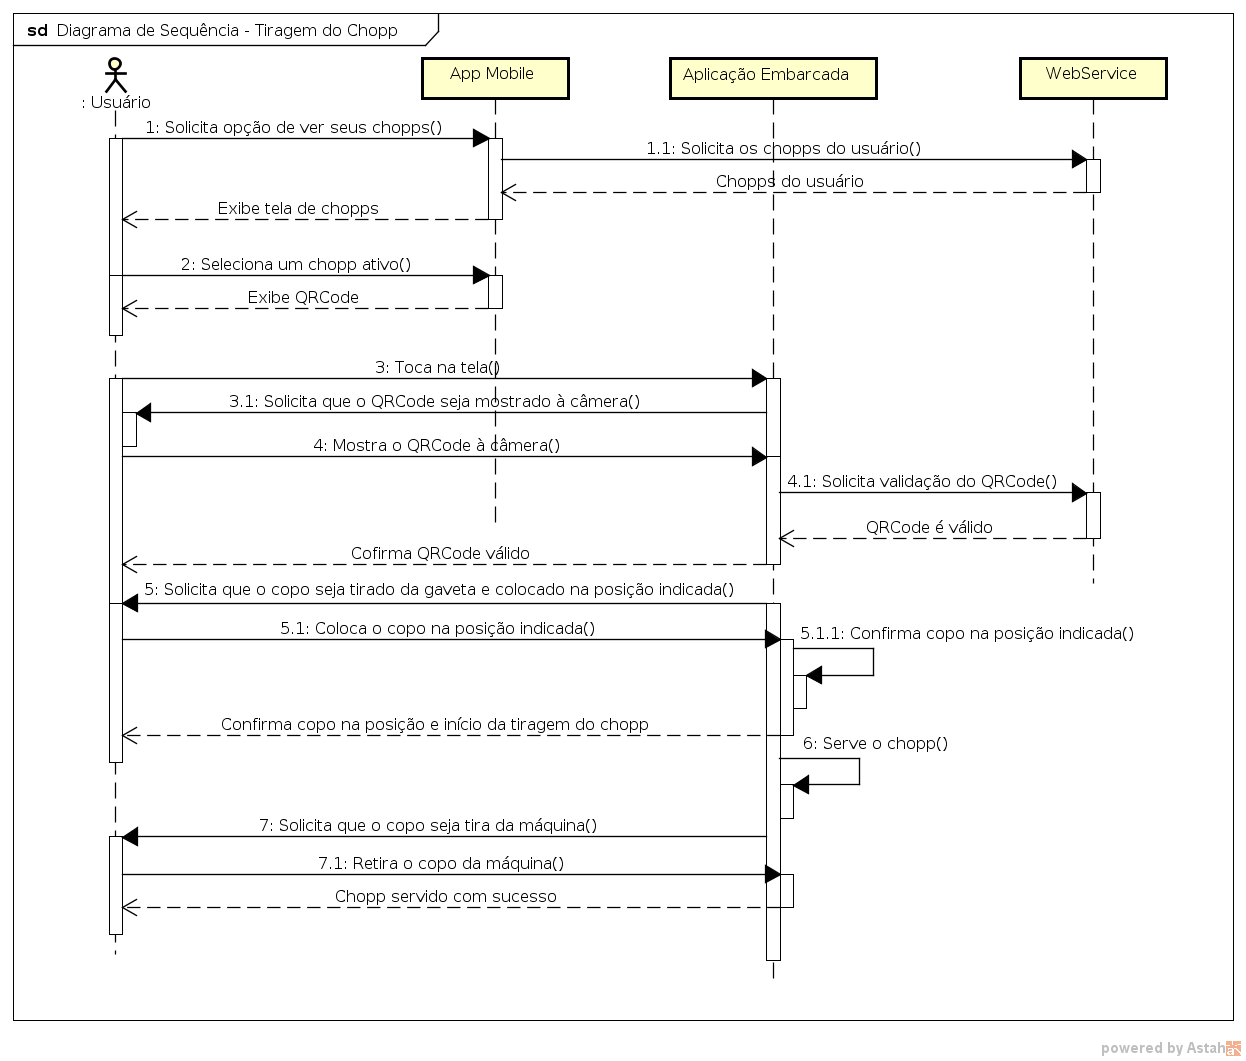
\includegraphics[scale= 0.4]{figuras/Diagrama-de-Sequencia-Tiragem-do-Chopp.png}        
    \caption{Diagrama de Sequência - Tiragem do Chopp. Fonte: Própria.}
    \label{classes-kivy}
\end{figure}

